% Options for packages loaded elsewhere
\PassOptionsToPackage{unicode}{hyperref}
\PassOptionsToPackage{hyphens}{url}
%
\documentclass[
]{article}
\usepackage{amsmath,amssymb}
\usepackage{lmodern}
\usepackage{iftex}
\ifPDFTeX
  \usepackage[T1]{fontenc}
  \usepackage[utf8]{inputenc}
  \usepackage{textcomp} % provide euro and other symbols
\else % if luatex or xetex
  \usepackage{unicode-math}
  \defaultfontfeatures{Scale=MatchLowercase}
  \defaultfontfeatures[\rmfamily]{Ligatures=TeX,Scale=1}
\fi
% Use upquote if available, for straight quotes in verbatim environments
\IfFileExists{upquote.sty}{\usepackage{upquote}}{}
\IfFileExists{microtype.sty}{% use microtype if available
  \usepackage[]{microtype}
  \UseMicrotypeSet[protrusion]{basicmath} % disable protrusion for tt fonts
}{}
\makeatletter
\@ifundefined{KOMAClassName}{% if non-KOMA class
  \IfFileExists{parskip.sty}{%
    \usepackage{parskip}
  }{% else
    \setlength{\parindent}{0pt}
    \setlength{\parskip}{6pt plus 2pt minus 1pt}}
}{% if KOMA class
  \KOMAoptions{parskip=half}}
\makeatother
\usepackage{xcolor}
\usepackage[margin=1in]{geometry}
\usepackage{graphicx}
\makeatletter
\def\maxwidth{\ifdim\Gin@nat@width>\linewidth\linewidth\else\Gin@nat@width\fi}
\def\maxheight{\ifdim\Gin@nat@height>\textheight\textheight\else\Gin@nat@height\fi}
\makeatother
% Scale images if necessary, so that they will not overflow the page
% margins by default, and it is still possible to overwrite the defaults
% using explicit options in \includegraphics[width, height, ...]{}
\setkeys{Gin}{width=\maxwidth,height=\maxheight,keepaspectratio}
% Set default figure placement to htbp
\makeatletter
\def\fps@figure{htbp}
\makeatother
\setlength{\emergencystretch}{3em} % prevent overfull lines
\providecommand{\tightlist}{%
  \setlength{\itemsep}{0pt}\setlength{\parskip}{0pt}}
\setcounter{secnumdepth}{-\maxdimen} % remove section numbering
\newlength{\cslhangindent}
\setlength{\cslhangindent}{1.5em}
\newlength{\csllabelwidth}
\setlength{\csllabelwidth}{3em}
\newlength{\cslentryspacingunit} % times entry-spacing
\setlength{\cslentryspacingunit}{\parskip}
\newenvironment{CSLReferences}[2] % #1 hanging-ident, #2 entry spacing
 {% don't indent paragraphs
  \setlength{\parindent}{0pt}
  % turn on hanging indent if param 1 is 1
  \ifodd #1
  \let\oldpar\par
  \def\par{\hangindent=\cslhangindent\oldpar}
  \fi
  % set entry spacing
  \setlength{\parskip}{#2\cslentryspacingunit}
 }%
 {}
\usepackage{calc}
\newcommand{\CSLBlock}[1]{#1\hfill\break}
\newcommand{\CSLLeftMargin}[1]{\parbox[t]{\csllabelwidth}{#1}}
\newcommand{\CSLRightInline}[1]{\parbox[t]{\linewidth - \csllabelwidth}{#1}\break}
\newcommand{\CSLIndent}[1]{\hspace{\cslhangindent}#1}
\usepackage{booktabs}
\usepackage{longtable}
\usepackage{array}
\usepackage{multirow}
\usepackage{wrapfig}
\usepackage{float}
\usepackage{colortbl}
\usepackage{pdflscape}
\usepackage{tabu}
\usepackage{threeparttable}
\usepackage{threeparttablex}
\usepackage[normalem]{ulem}
\usepackage{makecell}
\usepackage{xcolor}
\ifLuaTeX
  \usepackage{selnolig}  % disable illegal ligatures
\fi
\IfFileExists{bookmark.sty}{\usepackage{bookmark}}{\usepackage{hyperref}}
\IfFileExists{xurl.sty}{\usepackage{xurl}}{} % add URL line breaks if available
\urlstyle{same} % disable monospaced font for URLs
\hypersetup{
  pdftitle={The report of dropout prediction},
  pdfauthor={Ziyi Chen},
  hidelinks,
  pdfcreator={LaTeX via pandoc}}

\title{The report of dropout prediction}
\author{Ziyi Chen}
\date{2022-11-25 (updated: 2022-11-26)}

\begin{document}
\maketitle

{
\setcounter{tocdepth}{2}
\tableofcontents
}
\hypertarget{library-used}{%
\section{Library used}\label{library-used}}

\hypertarget{summary}{%
\section{Summary}\label{summary}}

Classification task performed through machine learning algorithms deals
which recognizing and grouping ideas into categories. These algorithms
are used to detect patterns within existing datasets to help classify
unseen and upcoming data. In this project 3 classification algorithms,
\texttt{Naive\ Bayes}, \texttt{Logistic\ Regression},
\texttt{Random\ Forest\ Classifier} were used on a real-life dataset, to
solve a two class classification problem. The performance of these 3
algorithms was compared through the classification metrics of
\texttt{Recall} and \texttt{F1\ score}. The
\texttt{Random\ Forest\ Classifier} and \texttt{Logistic\ Regression}
algorithms performed appreciably with a high recall score of 0.95 and
0.94 respectively. The selection and further optimization of the best
performing algorithm is planned for the future milestones of this
project.

\hypertarget{introduction}{%
\section{Introduction}\label{introduction}}

Academic performance/graduation in a population is an important factor
in their overall employability which contributes towards economic
development.Student Dropout given the factors on demography,
socioeconomics, macroeconomics, and relevant academic data provided by
the Student on enrollment. This prediction is important to understand
the student's academic capacity. This important knowledge can be used to
identify key areas of development such as the development of socially
disadvantaged communities, improvement of academic programs, development
of educational funding programs, etc. This project will try to
investigate the following research questions: 1. Given a student with
his/her demography, socioeconomics, macroeconomics, and relevant
academic data, how accurately can we predict whether he/she will drop
out of school? 2. What are the main factors contributing to the student
dropout rate?

\hypertarget{methods}{%
\section{Methods}\label{methods}}

\hypertarget{data}{%
\subsection{Data}\label{data}}

The dataset used in the project contains data collected at the time of
student enrollment and a snapshot of their performance at the end of the
2nd semester at their respective Universities. This includes discrete
and continuous data that capture the various facets of the student.
These include macroeconomic factors of inflation, GDP, and the
unemployment rate. It covers the personal/family details of the student
such as gender, previous grade, educational special needs, financial
status, parents' education, and parents' occupation. It captures aspects
of the educational system such as coursework enrolled, day/evening
classes, scholarships offered, etc. The dataset is created by Valentim
Realinho, Mónica Vieira Martins, Jorge Machado, and Luís Baptista from
the Polytechnic Institue of Portalegre. It was sourced from the UCI
Machine Learning Repository and can be downloaded from
\href{https://archive-beta.ics.uci.edu/dataset/697/predict+students+dropout+and+academic+success}{here}.
Each row represents the details pertaining to an individual student and
there are no duplicates.

The original dataset exhibits three classifications (class) of students
- Graduate, Enrolled, and Dropout. For the binary classification
question pursued in this project, the class Enrolled is omitted from the
dataset. The preliminary EDA shows there are 2209 examples of Graduate
students and 1421 examples of Dropouts. Thus the dataset imbalance is
not a major concern and can be addressed through balancing techniques
learned in the MDS program.

\hypertarget{analysis}{%
\subsection{Analysis}\label{analysis}}

\hypertarget{modeling}{%
\subsubsection{Modeling}\label{modeling}}

The insights gained from the EDA, provided a foundation to explore
multiple classification algorithms. Naive Bayes, Logistic Regression and
Random Forest Classifier were implemented for their respective
advantages in machine learning projects. These three algorithms provide
a nice selection on the spectrum of simple (Naive Bayes) to more complex
(Random Forest Classifier) algorithm. The Naive Bayes algorithm is
advantageous as a simple probabilistic classification algorithm which
assumes naively the independence between the features. Despite this
assumption, the Naive Bayes algorithm known to be perform well on
classification problems. The absence of hyperparameters and the
convenient scalability with increase in training dataset, made Naive
Bayes algorithm a favorable choice for this project. However, Naive
Bayes algorithm falls short in terms of interpretability of features
based on results. This is where the Logistic Regression algorithm shines
with its ability to provide interpretable feature importances while
retaining the model simplicity. The model parameters of
\texttt{class\ weight} and the \texttt{regularization\ (inverse)\ C}
were utilized to iteratively tune the performance. However Logistic
Regression assumes there is inherent linearity between our features and
the classification target. We are interested to implement an algorithm
which overcomes this limitation and this led us to the selection of the
Random Forest Classifier algorithm. Random Forest Classifier leverages
ensemble learning through multiple Decision Trees, which reduces the
tendency of overfitting to the training data. This is especially useful
when the number of records (train examples) are limited as is the case
in our project. This made Random Forest a favorable choice for our
project. The parameters of \texttt{max\_features}, \texttt{max\_depth},
\texttt{min\_samples\_leaf}, and \texttt{min\_samples\_leaf} were
optimized through \texttt{RandomSearchCV}. The Python 3 programming
language (Van Rossum and Drake Jr 1995) and the following Python
packages were used to perform the analysis: Scikit-learn (Pedregosa et
al. 2011), Numpy (Harris et al. 2020), Pandas (McKinney et al. 2010),
Seaborn (Waskom et al. 2017), Altair(VanderPlas et al. 2018),
Matplotlib(Tosi 2009); And the following external resources: The Origins
of Logistic Regression (Cramer 2002), Random Forests (Breiman 2001),
Predict students' dropout and academic success data set (V. M. Realinho
Valentim 2021), related research article (V. Realinho et al. 2022)

The code to perform the analysis and create the report can be found
\href{https://github.com/UBC-MDS/dropout-predictions}{here}

\hypertarget{results-discussion}{%
\section{Results \& Discussion}\label{results-discussion}}

\hypertarget{eda}{%
\subsection{EDA}\label{eda}}

\begin{figure}
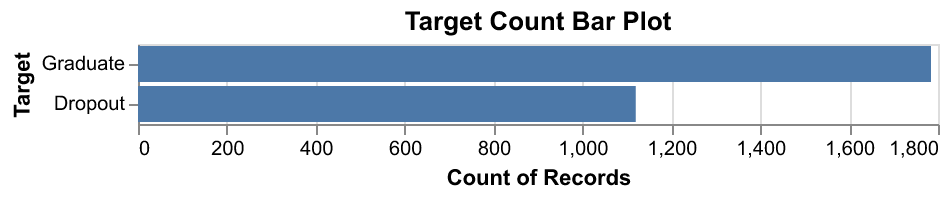
\includegraphics[width=1\linewidth]{../results/target_count_bar_plot} \caption{Figure 1. Visualization of targets of three categories.}\label{fig:target_count_bar_plot}
\end{figure}

From the above plot, we can see this problem was a three-category
classification task, and there exists a strong imbalance between those
three classes. The class Graduate has the majority count which is around
50\% of the records and Dropout has 32\% of the total records. The
Enrolled only has 18\% of the total records. Thus, during our training,
we need to find a way to fix this imbalance issue, possible solution
would be setting the \texttt{class\_weight} in our model. We decide to
drop one category which is enrolled student and only focus on graduate
\& dropout students to train our models.After dropping the Enrolled
students, we have around 60\% graduated students and 40\% dropout
students.

\begin{figure}
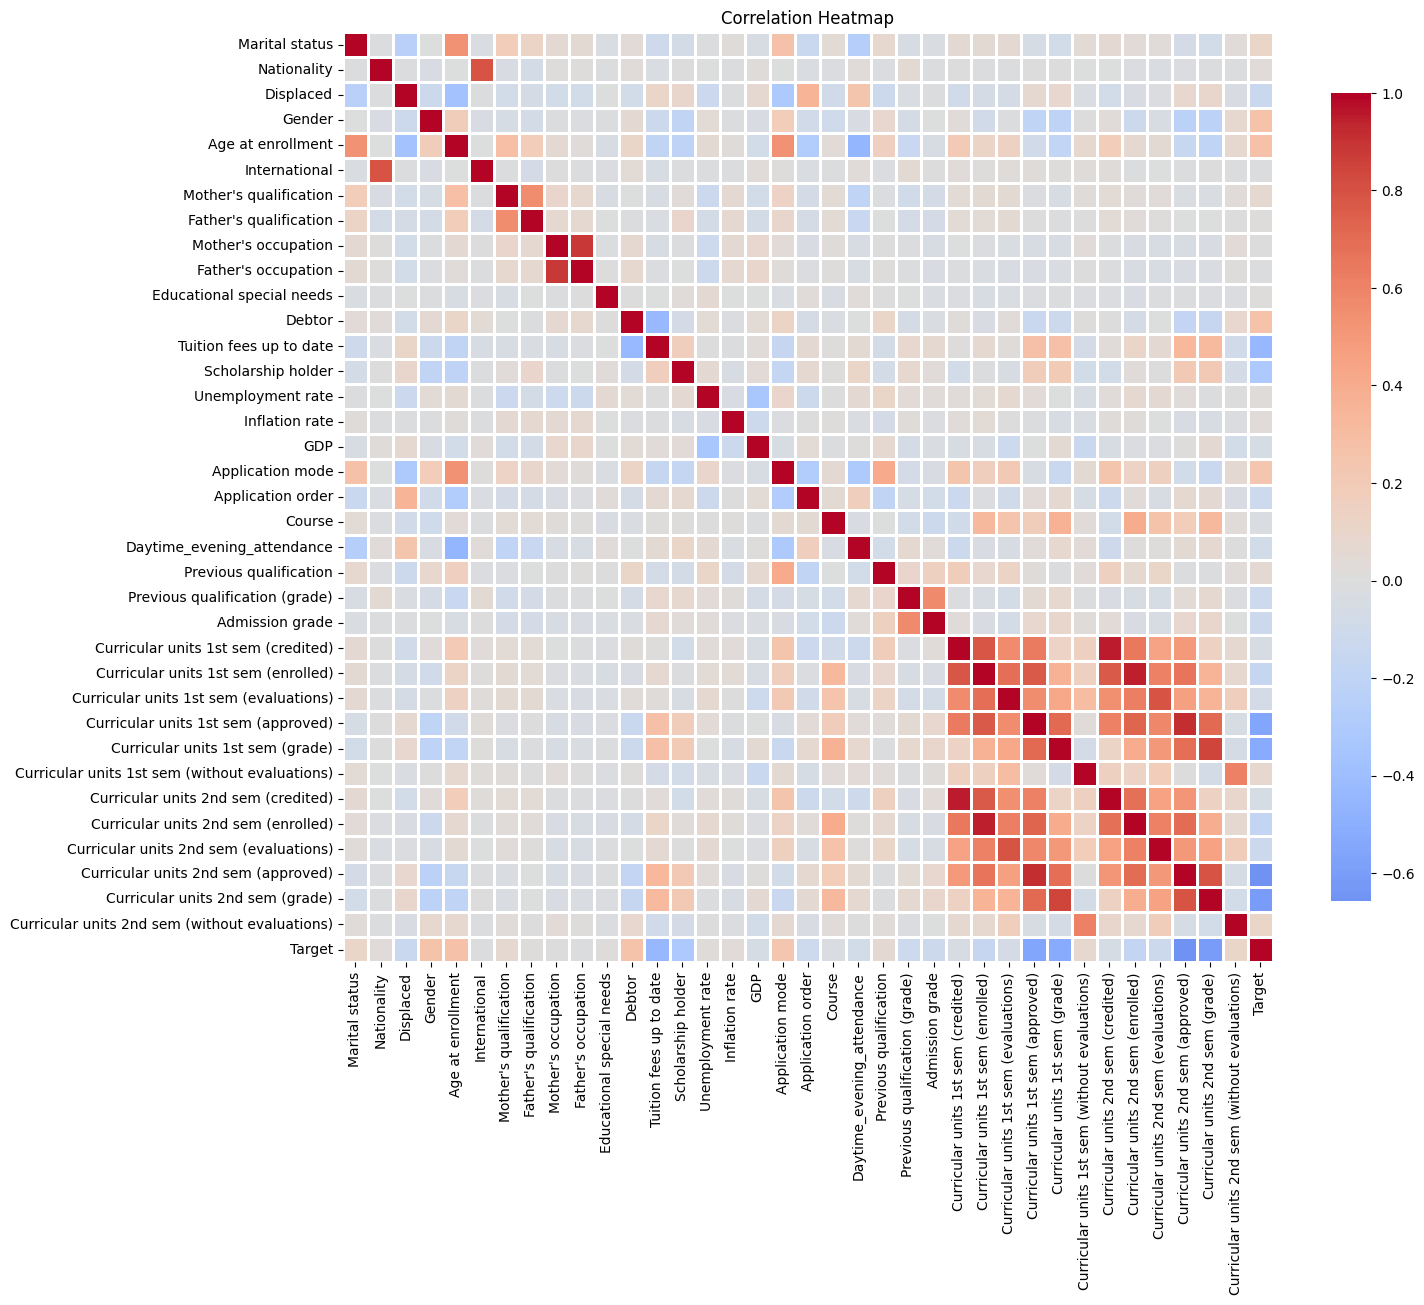
\includegraphics[width=1\linewidth]{../results/correlation_heatmap_plot} \caption{Figure 2. Heatmap of correlation across all features.}\label{fig:correlation_heatmap_plot}
\end{figure}

From the correlation heatmap, we can observe that some features are
strongly correlated (the dark red color), for example, Nationality \&
International, Age at enrollment \& Application mode. There are some
features with negative correlation, for example, Age at enrollment \&
Daytime Evening Attendance. In the following sections, we would like to
further investigate those positively correlated features, and features
in different potential categories (Demographic, Macroeconomic, Academic
data at enrollment, etc.).

\begin{figure}
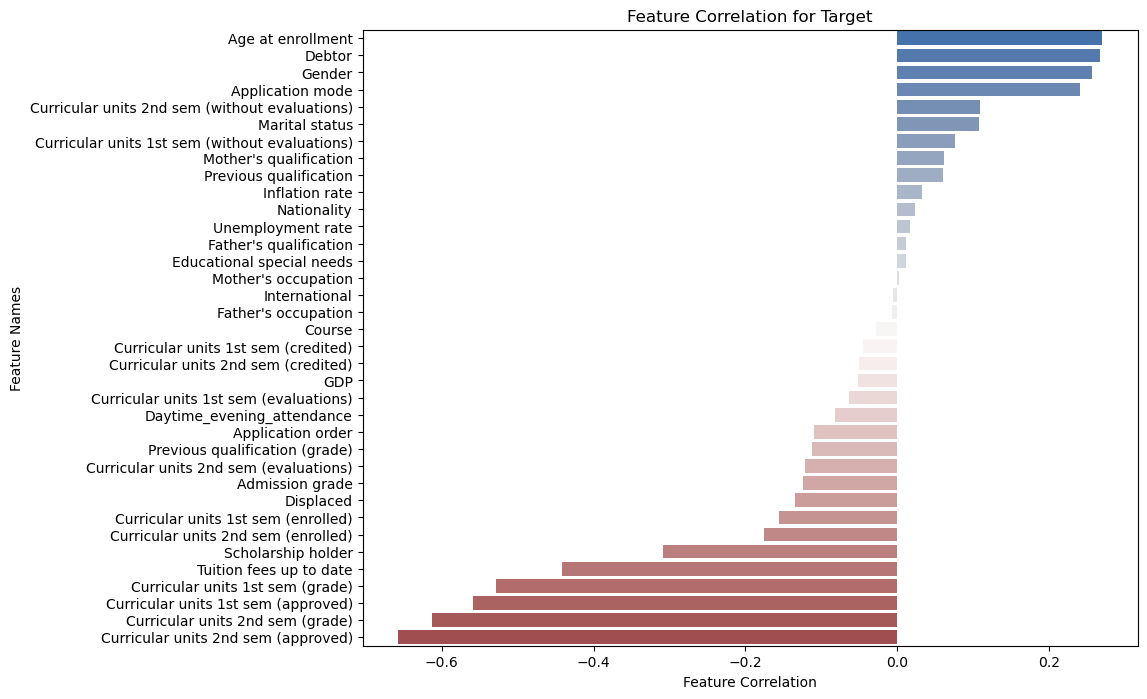
\includegraphics[width=1\linewidth]{../results/correlation_with_target_plot} \caption{Figure 3. Bar plot of feature correlation for target.}\label{fig:correlation_with_target_plot}
\end{figure}

There are more negatively correlated features than positives one. The
top 3 positively correlated features are \texttt{Age\ at\ enrollment},
\texttt{Debtor}, and \texttt{Gender}. In the below data exploration, we
can further investigate their relationship.

\begin{figure}
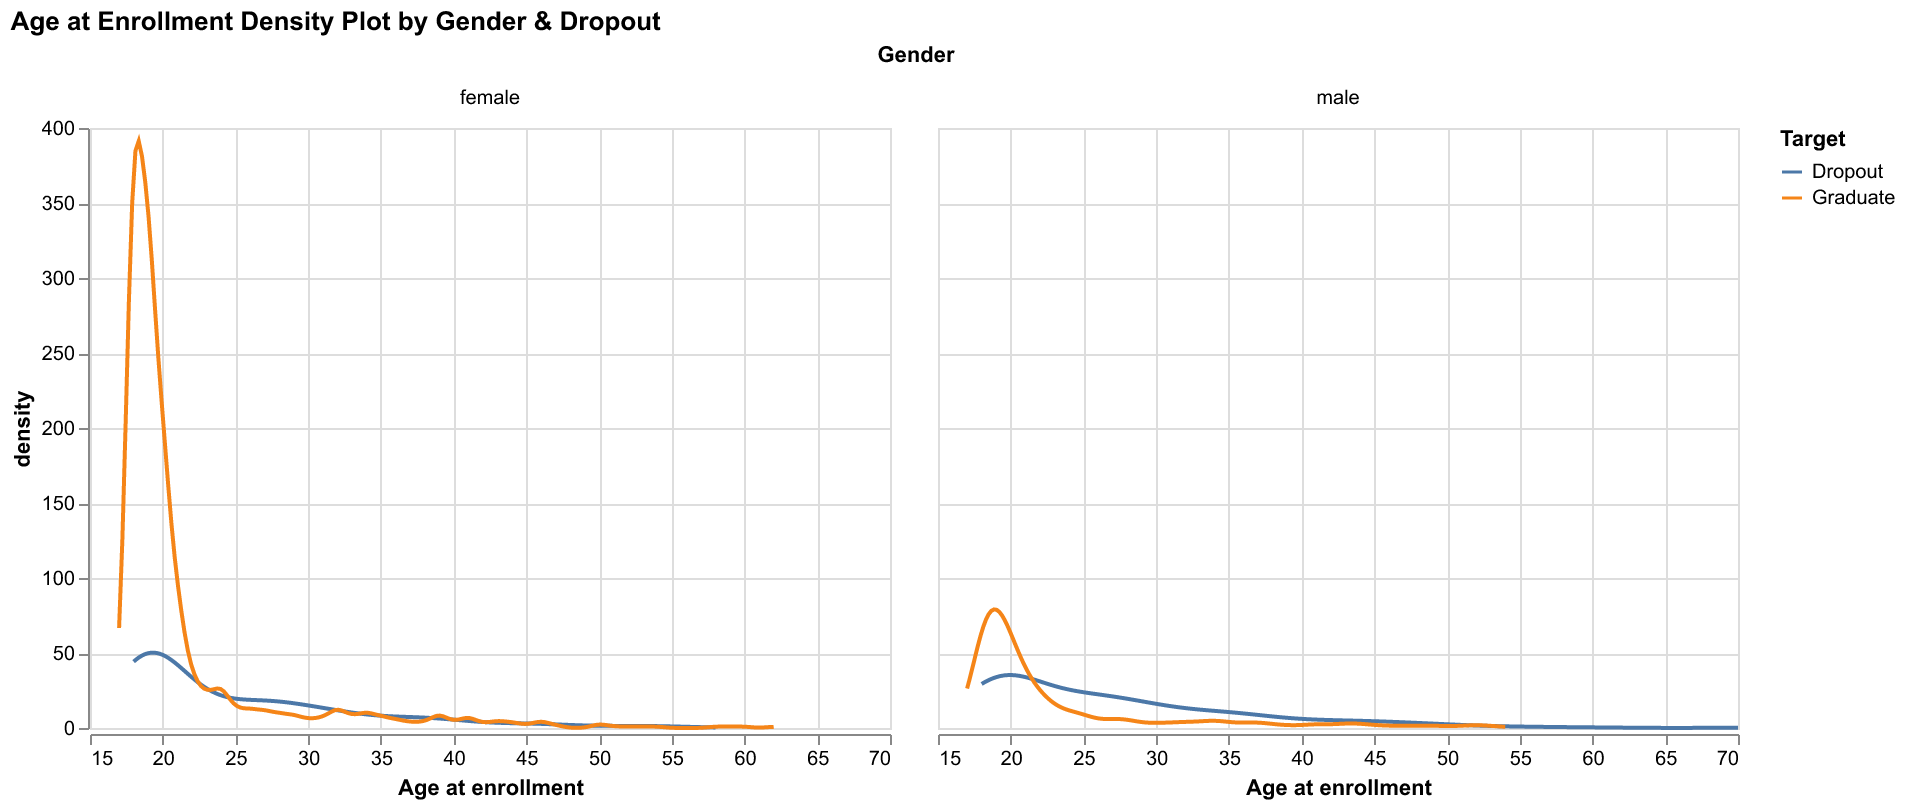
\includegraphics[width=1\linewidth]{../results/gender_density_plot} \caption{Figure 4. Density plot of different ages with enrollment by gender.}\label{fig:gender_density_plot}
\end{figure}

The density plot reveals the gender imbalance in our data set with the
number of younger female students than males. More male student aged 25
to 30 tends to drop out than females. While the students after their
30s, both gender demonstrate similar patterns.

\hypertarget{modeling-1}{%
\subsection{Modeling}\label{modeling-1}}

The objective of this project is to investigate how accurately we can
predict that a student will drop out of school. Furthermore what
underlying factors are the predominant influencing this outcome?
Accurate classification of a true drop out in the available data is our
chosen metric of interest. This is defined as \texttt{Recall} and it
represents the proportion of the true drop-outs in the dataset,
accurately predicted by the model. Each of the three models Naive Bayes,
Logistic Regression and Random Forest Classifier were fitted on training
data. The hyperparameter tuning was performed on using
\texttt{Random\ Search\ CV} for Logistic Regression and Random Forest
Classifier. The optimized models were then used to predict the
classification on the test data. The performance of the models was
compared through the Confusion Matrix, Precision-Recall curve, and
Receive-Operating Characteristics plots. The metrics were tabulated for
numerical interpretation.

Our train-test split yielded 726 examples in the testing dataset. There
are 425 actual class \texttt{Dropout} and the rest are
\texttt{Graduate}. The classification as a \texttt{Dropout} is
considered a True Positive in the context of this project. The
\texttt{Random\ Forest\ Classifier} model identified the highest True
positives among the three models (402) and achieved a superior recall
metric of 0.95. \texttt{Naive\ Bayes} model came close behind with 400
true positives at a recall metric of 0.94. The
\texttt{Logistic\ Regression} model achieved an appreciable recall
metric of 0.91 with 386 true positive.

The \texttt{Random\ Forest\ Classifier} and
\texttt{Logistic\ Regression} performed appreciably on the \texttt{f1}
score which is a balanced measure of model \texttt{precision} and
\texttt{recall}. However Naive Bayes suffered a relative low \texttt{f1}
score due to a low \texttt{precision}. This is due to more False
Positives predicted by \texttt{Naive\ Bayes} than the other models. The
corresponding confusion matrices derived from the analysis are shown
below for reference.

\begin{table}

\caption{\label{tab:load model test results}Table 1. Testing Score Results}
\centering
\begin{tabular}[t]{l|r|r|r}
\hline
Item & LogisticRegression & NaiveBayes & RandomForest\\
\hline
Recall & 0.8338870 & 0.6644518 & 0.8039867\\
\hline
Precision & 0.8655172 & 0.8888889 & 0.9132075\\
\hline
F1 & 0.8494078 & 0.7604563 & 0.8551237\\
\hline
Accuracy & 0.8774105 & 0.8264463 & 0.8870523\\
\hline
\end{tabular}
\end{table}

\begin{figure}
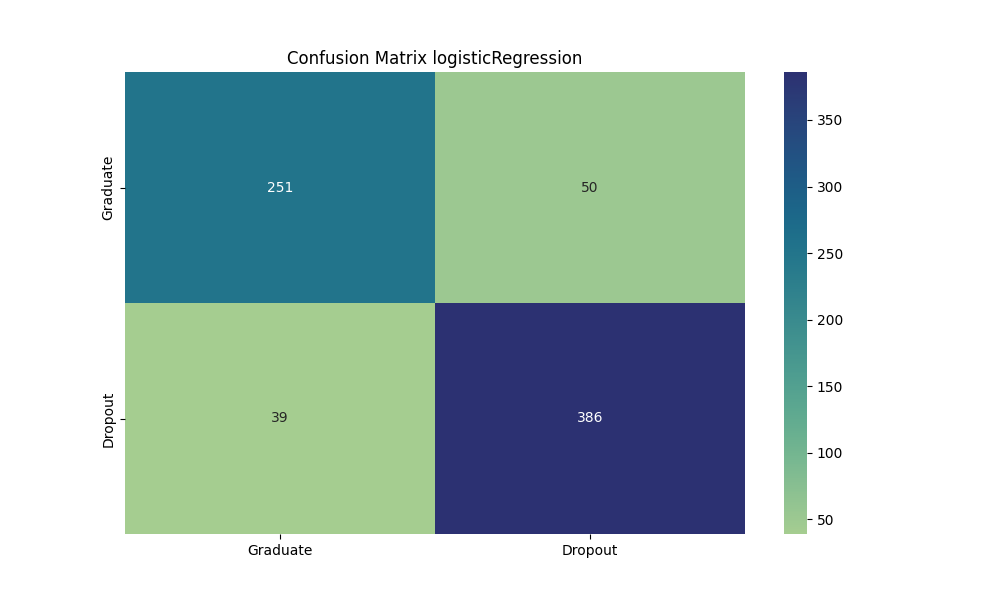
\includegraphics[width=1\linewidth]{../results/Confusion_Matrix_logisticRegression} \caption{Figure 5. Confusion matrix for Logistic Regression.}\label{fig:Confusion_Matrix_logisticRegression}
\end{figure}

\begin{figure}
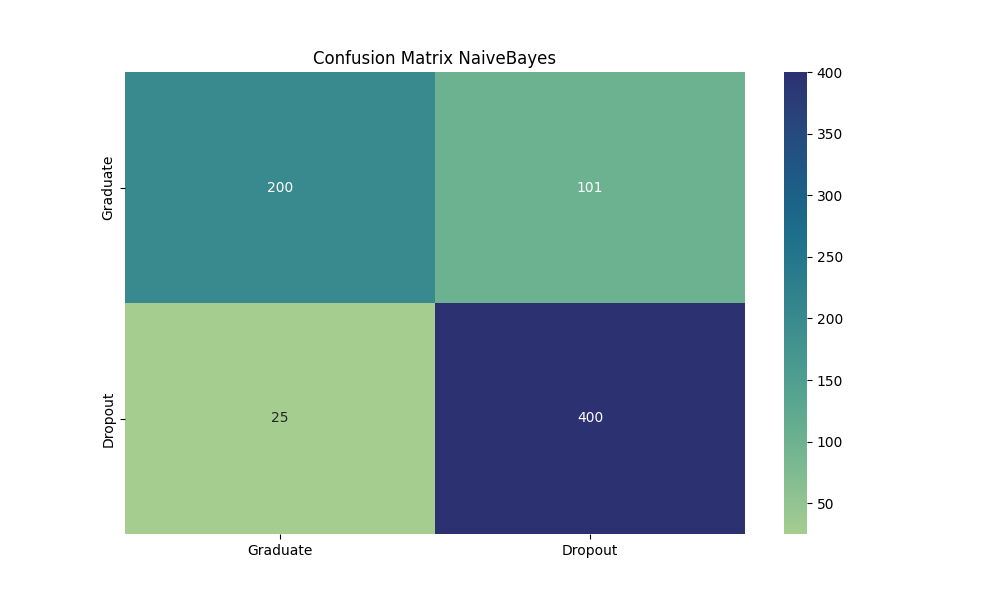
\includegraphics[width=1\linewidth]{../results/Confusion_Matrix_NaiveBayes} \caption{Figure 6. Confusion matrix image for Naive Bayes.}\label{fig:Confusion_Matrix_NaiveBayes}
\end{figure}

\begin{figure}
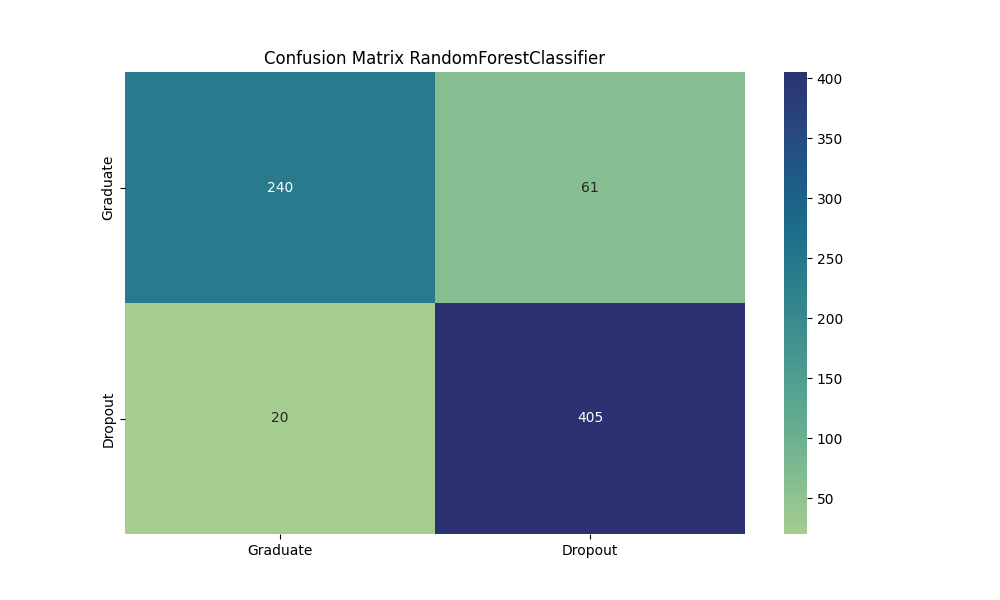
\includegraphics[width=1\linewidth]{../results/Confusion_Matrix_RandomForestClassifier} \caption{Figure 7. Confusion matrix image for RandomForest.}\label{fig:Confusion_Matrix_RandomForestClassifier}
\end{figure}

The performance of the three models can be visually inferred through the
\texttt{Precision-Recall} plot and the \texttt{ROC-AUC} plot. Both the
plots agree with our inferences from the confusion matrices. The
\texttt{Logistic\ Regression} model provides the best combination of
Precision and Recall for specific thresholds that can be leveraged to
further improve the model performance. The area under the
\texttt{ROC-AUC} plot is a measure of the model performance. The
\texttt{Naive\ Bayes} model is out clearly performed by the other two
models. The metrics are are tabulated below for reference.

\begin{figure}
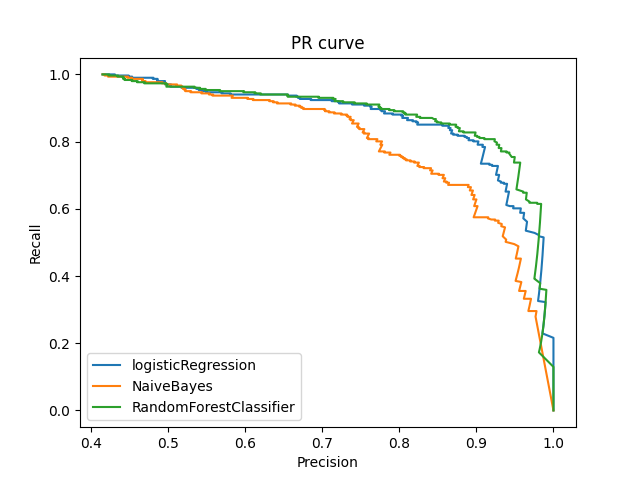
\includegraphics[width=1\linewidth]{../results/PR_curve} \caption{Figure 8. Precision and Recall Curve.}\label{fig:PR_curve}
\end{figure}

\begin{figure}
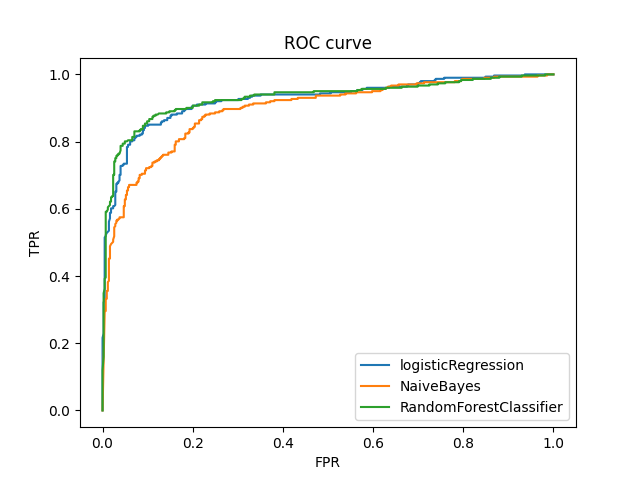
\includegraphics[width=1\linewidth]{../results/ROC_curve} \caption{Figure 9. ROC (receiver operating characteristic) Curve.}\label{fig:ROC_curve}
\end{figure}

\begin{table}

\caption{\label{tab:load model results}Table 2. Cross Validation Results}
\centering
\begin{tabular}[t]{l|l|l|l|l|l|l}
\hline
Item & LogisticRegression & LogisticRegression & NaiveBayes & NaiveBayes & RandomForest & RandomForest\\
\hline
NA & mean & std & mean & std & mean & std\\
\hline
fit\_time & 0.187 & 0.009 & 0.002 & 0.0 & 1.542 & 0.083\\
\hline
score\_time & 0.0 & 0.0 & 0.001 & 0.0 & 0.013 & 0.008\\
\hline
test\_score & 0.841 & 0.019 & 0.729 & 0.055 & 0.822 & 0.019\\
\hline
train\_score & 0.85 & 0.007 & 0.73 & 0.053 & 0.859 & 0.008\\
\hline
\end{tabular}
\end{table}

The current analysis is performed using the features selected post EDA
through human judgement based on the project context. Both the models
\texttt{Logistic\ Regression} and \texttt{Random\ Forest\ Classifier}
have a small number of False Negatives. These are students who are
actually \texttt{Dropout} but were incorrectly classified as
\texttt{Graduate} by the models. In the context of this project, it is
our endeavor to minimize these False Negatives as much as possible. The
further steps will involve investigative methodologies such as
\texttt{Feature\ Selection} and \texttt{Feature\ Engineering} to reduce
the False Negatives and further improve the performance.

\hypertarget{references}{%
\section*{References}\label{references}}
\addcontentsline{toc}{section}{References}

\hypertarget{refs}{}
\begin{CSLReferences}{1}{0}
\leavevmode\vadjust pre{\hypertarget{ref-breiman2001random}{}}%
Breiman, Leo. 2001. {``Random Forests.''} \emph{Machine Learning} 45
(1): 5--32.

\leavevmode\vadjust pre{\hypertarget{ref-cramer2002origins}{}}%
Cramer, Jan Salomon. 2002. {``The Origins of Logistic Regression.''}

\leavevmode\vadjust pre{\hypertarget{ref-harris2020array}{}}%
Harris, Charles R, K Jarrod Millman, Stéfan J Van Der Walt, Ralf
Gommers, Pauli Virtanen, David Cournapeau, Eric Wieser, et al. 2020.
{``Array Programming with NumPy.''} \emph{Nature} 585 (7825): 357--62.

\leavevmode\vadjust pre{\hypertarget{ref-mckinney2010data}{}}%
McKinney, Wes et al. 2010. {``Data Structures for Statistical Computing
in Python.''} In \emph{Proceedings of the 9th Python in Science
Conference}, 445:51--56. 1. Austin, TX.

\leavevmode\vadjust pre{\hypertarget{ref-pedregosa2011scikit}{}}%
Pedregosa, Fabian, Gaël Varoquaux, Alexandre Gramfort, Vincent Michel,
Bertrand Thirion, Olivier Grisel, Mathieu Blondel, et al. 2011.
{``Scikit-Learn: Machine Learning in Python.''} \emph{The Journal of
Machine Learning Research} 12: 2825--30.

\leavevmode\vadjust pre{\hypertarget{ref-realinho2022predicting}{}}%
Realinho, Valentim, Jorge Machado, Luı́s Baptista, and Mónica V Martins.
2022. {``Predicting Student Dropout and Academic Success.''} \emph{Data}
7 (11): 146.

\leavevmode\vadjust pre{\hypertarget{ref-misc_predict_students}{}}%
Realinho, Vieira Martins, Valentim. 2021. {``{Predict students' dropout
and academic success}.''} UCI Machine Learning Repository.

\leavevmode\vadjust pre{\hypertarget{ref-tosi2009matplotlib}{}}%
Tosi, Sandro. 2009. \emph{Matplotlib for Python Developers}. Packt
Publishing Ltd.

\leavevmode\vadjust pre{\hypertarget{ref-van1995python}{}}%
Van Rossum, Guido, and Fred L Drake Jr. 1995. \emph{Python Tutorial}.
Vol. 620. Centrum voor Wiskunde en Informatica Amsterdam, The
Netherlands.

\leavevmode\vadjust pre{\hypertarget{ref-vanderplas2018altair}{}}%
VanderPlas, Jacob, Brian Granger, Jeffrey Heer, Dominik Moritz, Kanit
Wongsuphasawat, Arvind Satyanarayan, Eitan Lees, Ilia Timofeev, Ben
Welsh, and Scott Sievert. 2018. {``Altair: Interactive Statistical
Visualizations for Python.''} \emph{Journal of Open Source Software} 3
(32): 1057.

\leavevmode\vadjust pre{\hypertarget{ref-waskom2017mwaskom}{}}%
Waskom, Michael, Olga Botvinnik, Drew O'Kane, Paul Hobson, Saulius
Lukauskas, David C Gemperline, Tom Augspurger, et al. 2017.
{``Mwaskom/Seaborn: V0. 8.1 (September 2017).''} \emph{Zenodo}.

\end{CSLReferences}

\end{document}
